\documentclass[a4paper, 12pt, oneside, dutch]{article}
\usepackage[T1]{fontenc}
\usepackage{aurical}
% Babel package:
\usepackage{babel}[dutch]
\usepackage{booktabs}
\usepackage{textalpha}
\usepackage{url}

\usepackage[dvipsnames]{xcolor}
\usepackage{eso-pic,graphicx}
\usepackage[top=40mm, bottom=58mm, outer=50mm, inner=50mm]{geometry}
\setlength{\columnsep}{90pt}

\definecolor{customColor}{RGB}{213, 246, 251}

\usepackage{sectsty}
\usepackage[titles]{tocloft}

\usepackage{setspace}
\onehalfspacing

\allsectionsfont{\Fontauri}
\sectionfont{\Fontauri\Huge}
\subsectionfont{\Fontauri\LARGE}
\subsubsectionfont{\Fontauri\Large}

\setlength{\emergencystretch}{15pt}
\usepackage{fancyhdr}
\usepackage{amssymb}
\usepackage{array}
\usepackage{imakeidx}
\usepackage{qtree}
\usepackage{microtype}
% change color of text, example replace all \color{Goldenrod} with \color{lightgray}

\makeatletter % change only the display of \thepage, but not \thepage itself:
\patchcmd{\ps@plain}{\thepage}{\bfseries\large\color{customColor}{\thepage}}{}{}
\makeatother

\color{customColor}

\begin{document}
\Fontauri
\renewcommand{\cftfigfont}{\Fontauri}
\renewcommand{\cftfigpagefont}{\Fontauri}

\renewcommand{\cftsecfont}{\Fontauri}
\renewcommand{\cftsubsecfont}{\Fontauri}
\renewcommand{\cftsubsubsecfont}{\Fontauri}
% fix toc page numbers
\let\origcftsecfont\cft
\let\origcftsecpagefont\cftsecpagefont
\let\origcftsecafterpnum\cftsecafterpnum
\renewcommand{\cftsecpagefont}{\Fontauri{\origcftsecpagefont}}
\renewcommand{\cftsecafterpnum}{\Fontauri{\origcftsecafterpnum}}
\let\origcftsubsecpagefont\cftsubsecpagefont
\let\origcftsubsecafterpnum\cftsubsecafterpnum
\renewcommand{\cftsubsecpagefont}{\Fontauri{\origcftsubsecpagefont}}
\renewcommand{\cftsubsecafterpnum}{\Fontauri{\origcftsubsecafterpnum}}
\let\origcftsubsubsecpagefont\cftsubsubsecpagefont
\let\origcftsubsubsecafterpnum\cftsubsubsecafterpnum
\renewcommand{\cftsubsubsecpagefont}{\Fontauri{\origcftsubsubsecpagefont}}
\renewcommand{\cftsubsubsecafterpnum}{\Fontauri{\origcftsubsubsecafterpnum}}

\renewcommand\thefootnote{\Fontauri{\arabic{footnote}}}
\let\oldfootnote\footnote
    \renewcommand{\footnote}[1]{\oldfootnote{\Fontauri\large#1}}
\AddToShipoutPictureBG{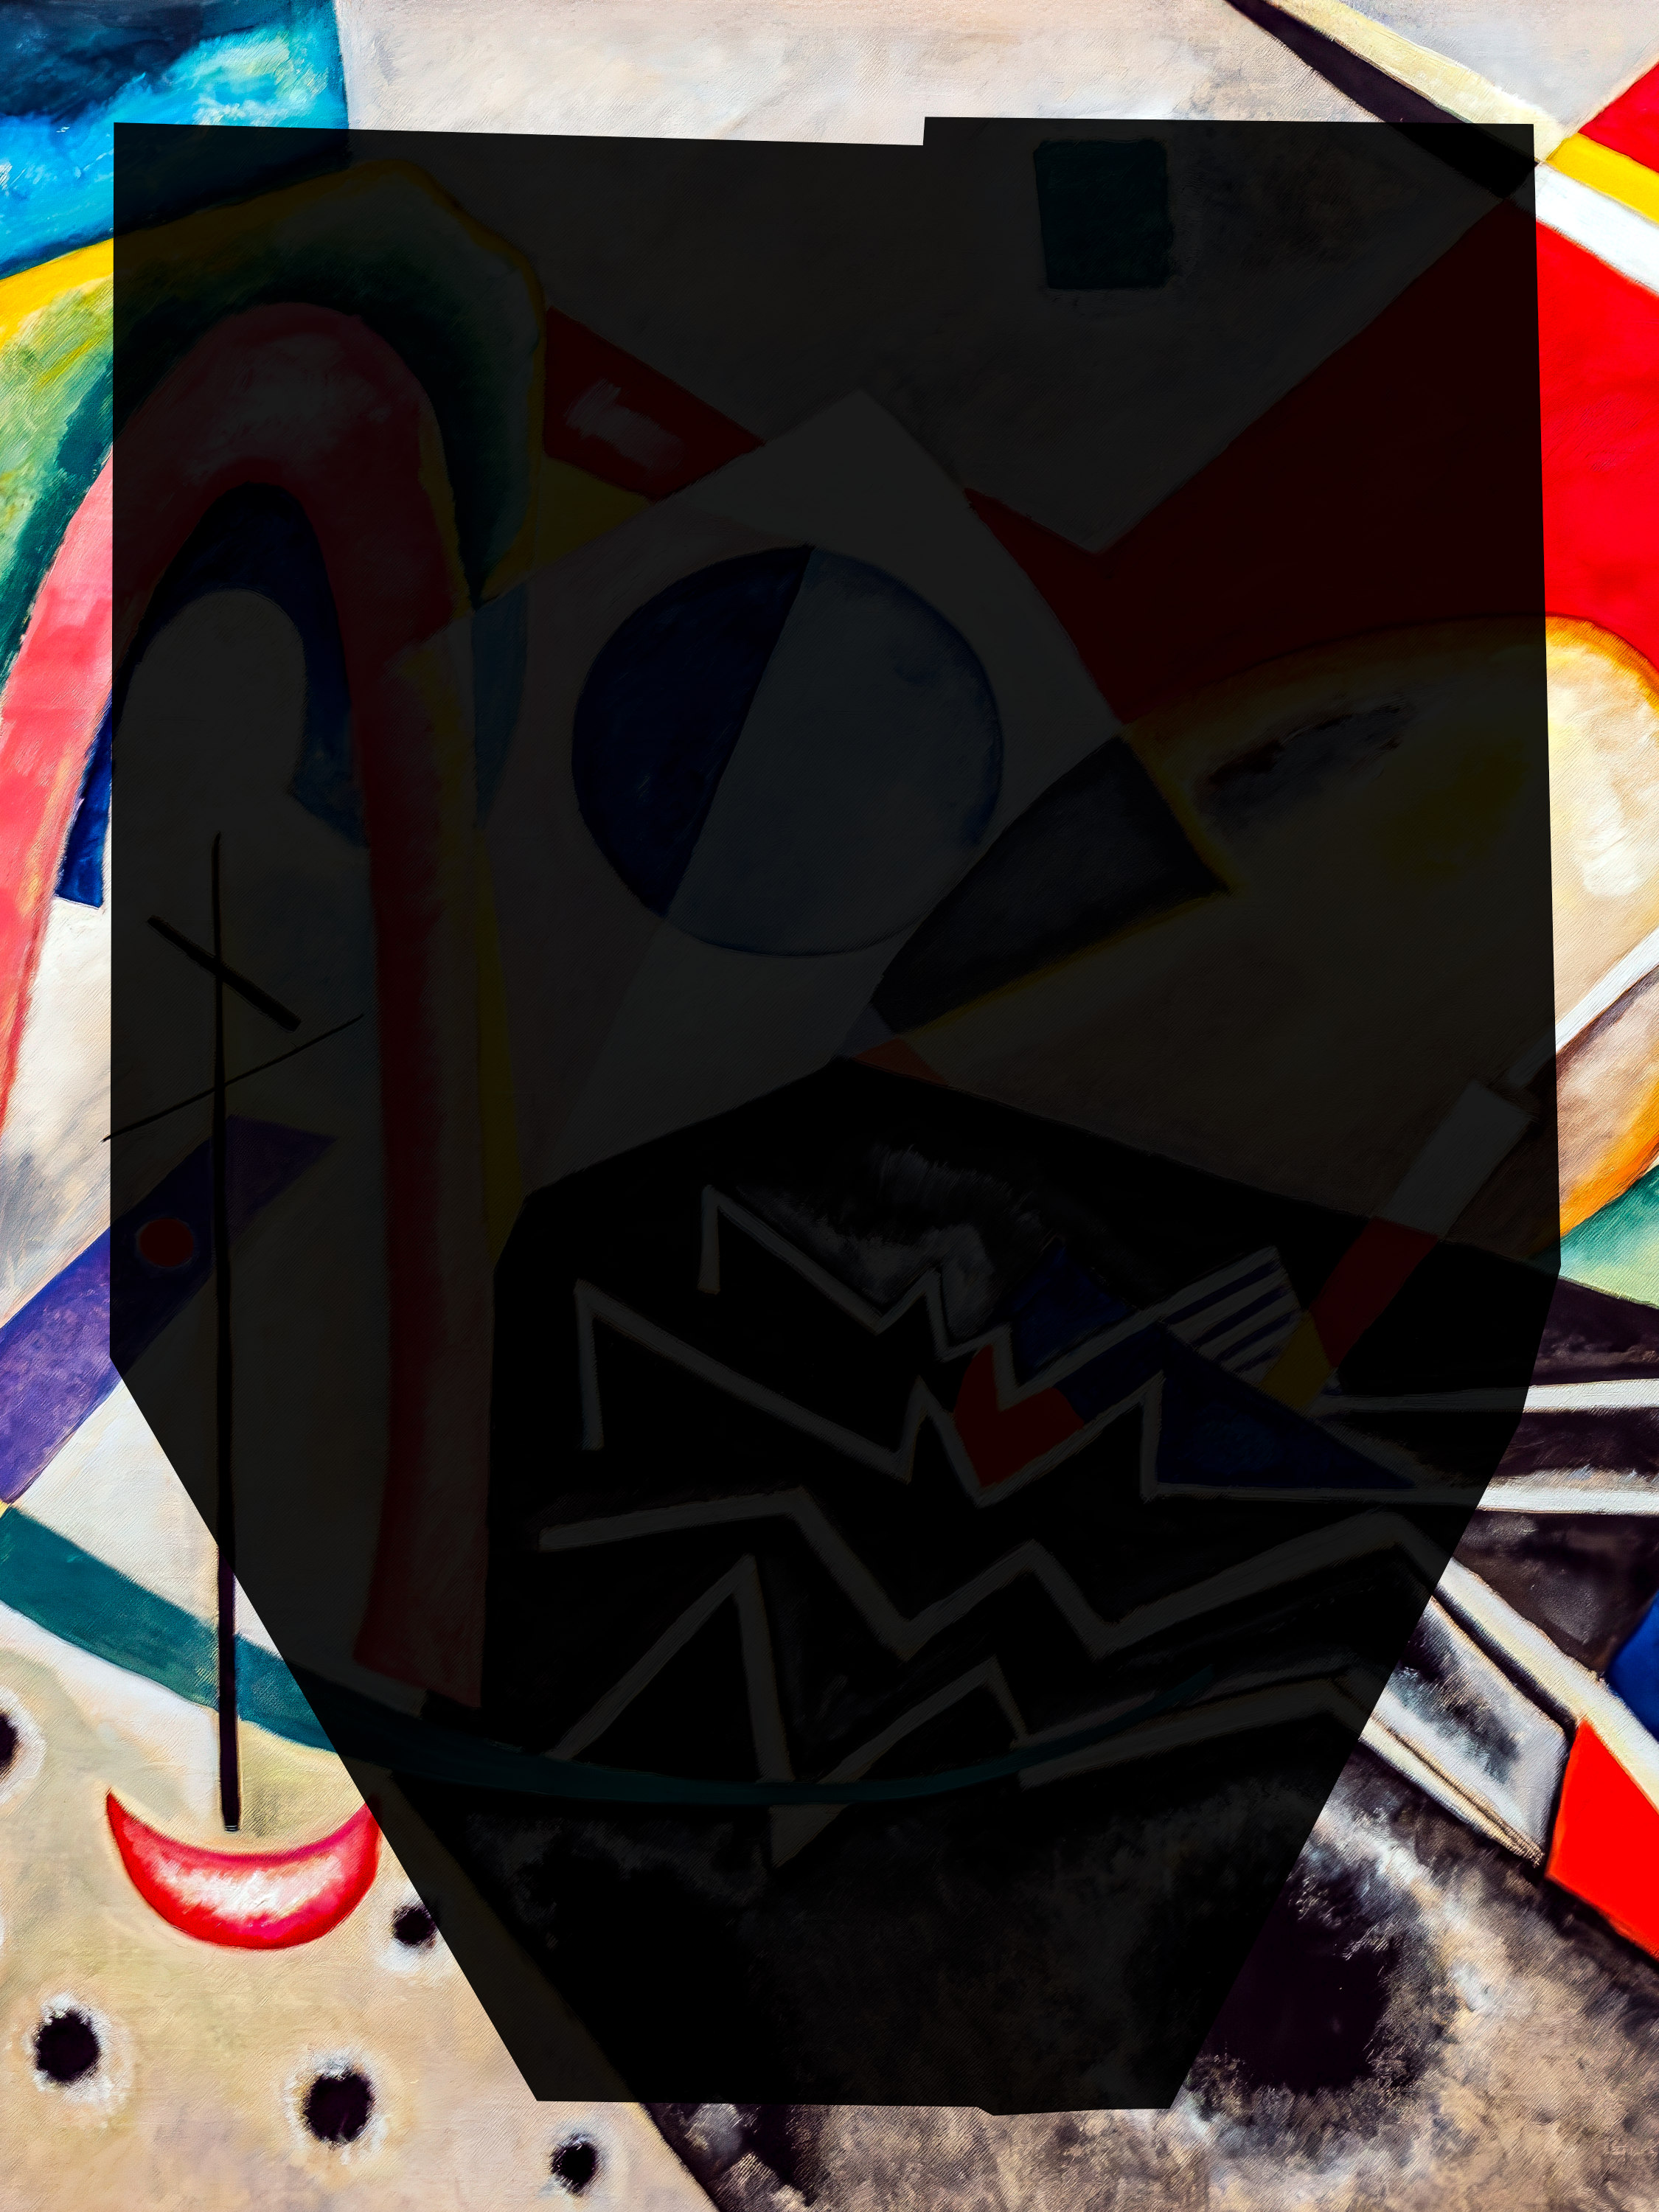
\includegraphics[width=\paperwidth,height=\paperheight]{abstract.jpeg}}
\begin{titlepage} % Suppresses headers and footers on the title page
	\centering % Centre everything on the title page
	\scshape % Use small caps for all text on the title page

	%------------------------------------------------
	%	Title
	%------------------------------------------------
	
	\rule{\textwidth}{1.6pt}\vspace*{-\baselineskip}\vspace*{2pt} % Thick horizontal rule
	\rule{\textwidth}{0.4pt} % Thin horizontal rule
	
	\vspace{0.75\baselineskip} % Whitespace above the title

        {\Huge Anarchie \\} % Title
	
	\vspace{0.75\baselineskip} % Whitespace below the title
	
	\rule{\textwidth}{0.4pt}\vspace*{-\baselineskip}\vspace{3.2pt} % Thin horizontal rule
	\rule{\textwidth}{1.6pt} % Thick horizontal rule
	
	\vspace{1\baselineskip} % Whitespace after the title block
	
	%------------------------------------------------
	%	Subtitle
	%------------------------------------------------
	
	{Door \scshape\Large Dr. Eugen Heinrich Schmitt,\\\emph{te Budapest} \\} % Subtitle or further description
	
	\vspace*{1\baselineskip} % Whitespace under the subtitle
	
	%------------------------------------------------
	%	Editor(s)
	%------------------------------------------------

 	% Subtitle or further description

	\vspace{1\baselineskip} % Whitespace before the editors

        {\small Vertaling van Dr. Louis A. Bähler.}

    %------------------------------------------------
	%	Cover photo
	%------------------------------------------------
	
	%\includegraphics[scale=1]{cover}
	
	%------------------------------------------------
	%	Publisher
	%------------------------------------------------
		
	\vspace*{\fill}% Whitespace under the publisher logo
	
	Amsterdam 1899 % Publication year
	
	{\small J. Sterringa } % Publisher

	\vspace{1\baselineskip} % Whitespace under the publisher logo

        Internet Archive Online Edition  % Publication year
	
	{\small Naamsvermelding-NietCommercieel-GelijkDelen 4.0 Internationaal } % Publisher
\end{titlepage}
\setlength{\parskip}{1mm plus1mm minus1mm}
\clearpage
\pagestyle{fancy}
\fancyhf{}
\cfoot{\Fontauri{\thepage}}
\Large
\paragraph{}
Als een woord der verschrikking klinkt dit woord tegenwoordig door de wereld.

En toch is de oorspronkelijke, zuivere, onvervalschte beteekenis van ditzelfde woord de verhevenste idee, die ooit in den geest der menschheid ontwaakt is, zijnde niet enkel een ideaal, maar --- zooals we zullen aantoonen --- de volheid van alle idealen, die ooit het menschelijk gemoed met verheffende gevoelens vervuld heeft. Ja, in werkelijkheid is dit verschrikkelijke woord het teederste woord. Het is de majesteit van het zelf bewustzijn en de vrede des geestes, de hemelsche bode die de opdracht heeft, deze van demonisch dierlijke hartstochten omwoelde, deze eeuwenlang met bloed en tranen bemeste aarde omtescheppen in een paradijs. In een paradijs waarin alle scheidsmuren zijn neergestort, die de menschheid verdeelen en waarin eene met Goddelijk albewustzijn vervulde, alles samensmeltende wereldbeschouwing onbeperkt den schepter voert.

De woorden, welke het Evangelie den Heiland der wereld toeschrijft nl.: "`Mijn last is licht en mijn juk is zacht"' --- zij gelden van deze goddelijke idee.

Want wat beteekent eigenlijk dit Grieksche woord anarchie? Letterlijk beteekent anarchie dat niemand de eerste, niemand heerscher mag wezen.
Het is het protest tegen iederen vorm van dwingelandij.

Ieder menschelijk gemoed dat goed en edel voelt, moet noodzakelijk in deze idee het ideaal zien van menschelijke samenleving. Wat toch dunkt u zoo harmonisch als een maatschappij die van allen uitwendigen dwang verlost is en enkel door inwendige drijfveeren vrijelijk hare bestaansvormen aanneemt. Treedt hier niet voor oogen hetgeen in waarheid hoog menschelijk is?

De twijfel en de bedenking die zich tegen deze idee keert, is daarom rechtstreeks twijfel aan de menschelijke natuur en wortelt in de opvatting dat de mensch oorspronkelijk niets dan een listig dier is en voor altoos door laag-zelfzuchtige beweegredenen van hebzucht en heerschzucht bewogen wordt; dat hij niet, tegenover zijn naaste, de edele, behulpzame en beschermende, zelfopofferende goddelijke mensch kan zijn, maar veeleer de ellendige, vraatzuchtige, onverzadelijke wolf (of juister nog jakhals) is en blijven moet; en dat dit eeuwig begeerige en eeuwig onverzadelijke beest, dat er niet slechts op loert om de bete van den naaste maar ook diens vleesch en bloed te verslinden, enkel in bedwang gehouden kan worden door de ijzeren roede van een uitwendig dwangbewind.

Onbetwistbaar blijft in de geschiedenis der menschheid tot nu toe dit treurige feit bestaan, dat, begunstigd door de onvolkomen productieverhoudingen, door onvoldoende beheersching van de natuur, welke zoowel de menschen als hunne werkkracht isoleerde en versnipperde, juist de wreedste, heerschzuchtigste, laag egoïstische lieden, die er 't minst bezwaar in zagen een medemensch te onderdrukken en te overweldigen, zich het zekerst en het gemakkelijkst tot macht en aanzien verhieven --- dat dus zij die eigenlijk de slechtsten en ellendigsten waren, de menschen die door hun bekrompen zelfzucht nog het dichtst bij het dier stonden, de roovers die op groote schaal wisten te werken en in bloedige onmeedoogendheid bij massa omtebrengen of te onderwerpen, het stelligst in de hoogte kwamen. Wie zich in den dierlijken strijd om het bestaan juist door deze eigenschappen of door sluwe, meedoogenlooze exploitatie van den goedwilligen medemensch uit de groote menigte naar boven wist te werken, geraakte zoo in 't algemeen tot heerschappij. Deze groote menigte zelve moest derhalve in 't algemeen, ingeval we den mensch niet den maatstaf van het dier maar den maatstaf van den mensch aanleggen, moest gemiddeld veel en veel beter en edeler geaard zijn dan dat ware schuim der menschheid dat boven kwam drijven in den grooten stroom der wereldgeschiedenis.

Men is gewoon, anarchie en terrorisme voor hetzelfde te houden en gaat dan uit van afdwalingen van enkele anarchisten, die naar de middelen van hunne tegenstanders grepen. Maar wat is onze organisatie van staat en maatschappij met hare millioenen bajonetten, geweren en kanonnen, met hare politie, rechtbanken, overheden, beulen en beulsknechten, met hare oorlogen, terechtstellingen, gevangenissen en verbanningen anders dan een organisatie die van onder tot boven berust op den schrik (Latijn: terror), dus op het terrorisme.

Daarom is het allerbelachelijkst, wanneer men onze staatsredders tegen het terrorisme hoort aangaan.

Het heerschende element in de geschiedenis, de heerschende orde, is tot den dag van heden juist het terrorisme geweest en de anarchie is in haar wortel eigenlijk de onvermoeide strijd tegen het heerschende terrorisme.

Daar nu de terroristen in 't algemeen de toestanden beheerschen, moest hun streven er eensdeels op gericht wezen, zulke opvattingen in hoofd en hart der onderdrukten te doen postvatten als in overeenstemming waren met de belangen van hunne heerschzucht en zelfzucht. Deze opvattingen hadden aan den eenen kant betrekking op hen zelven --- de heerschers ---, aan den anderen kant op de overheerschte menigte.

Wat henzelven betreft, zoo moest al hun streven daar op uitgaan om de inwendige holheid, de diepe, inwendige ellendigheid van deze egoïste, in hun dierlijk Ik opgesloten menschen door verblindende praal van buiten, door uiterlijken schijn te vermommen. Het monster moest prachtig uitgedost in koninklijk purper, in goud en zijde rondloopen; het moest verder, daar innerlijke, oprechte achting tegenover hem onmogelijk was, zich met de blinkende heerlijkheid van moordtuig omgeven, teneinde zoo den schrik en ontzetting in de menigte levendig te houden. Voorts moesten zij het er op toeleggen, dat de daden van het monster als heerlijke daden met den valschen schijn van zedelijke verhevenheid werden omluisterd.

Brutale, dierlijke, uitwendige macht moest voor eer moord op groote schaal voor roem, hartelooze, schaamtelooze hoogmoed en menschenverachting voor adel en zedelijke meerderheid doorgaan. In deze gestalte treden dan ook de meest oprechte en (in betrekkelijken zin gesproken) meest eerlijke van deze bandieten aan het licht. De sluwsten en huichelachtigsten onder hen zoeken echter hunne daden van geweld en verdrukking, hun moord en roof te bemantelen onder den mantel van menschenliefde en humaniteit.

Ten opzichte van de groote menigte nu vinden deze terroristen voor hun eigen roofzuchtig doen het beste voorwendsel en den schijn van rechtvaardiging hierin dat zij de groote menigte zoo laag mogelijk in de schatting van het publiek naar beneden duwen; dat zij in den mensch de hierboven beschreven wolvennatuur zien --- ofschoon deze beschrijving op de heer schenden zelven onvergelijkelijk veel beter van toepassing is. De vertegenwoordigers van die richting blijken ultra-realisten te zijn, want altijd weer leggen zij den nadruk op 's menschen onvolkomenheid, slechtheid en zwakheid, altijd weer wijzen zij op het beest in den mensch, ten einde voor hun boos geweten een soort verontschuldiging van hunne gewelddaden te verkrijgen.

De wereldbeschouwing, welke deze menschen er op na houden, beweegt zich weliswaar in twee lijnrechte tegenstellingen, doch in weerwil van den oogenschijnlijk onverzoenbaren strijd tusschen beide standpunten, zijn beide desniettemin in werkelijke overeenstemming ten opzichte van bovengenoemde levenspraktijk, hetgeen reeds hierom zoo moet wezen, omdat aan deze praktische levensrichting juist een bepaalde beschouwing over den mensch ten grondslag ligt. Deze beide tegenstellingen kunnen we noemen de wereldbeschouwing van de theologie en de wereldbeschouwing van het materialisme. Terwijl de theologie in de gestalte van een uitwendigen hemeldespoot de menschelijke heerschzucht, zelfzucht en wreedaardigheid in den hemel verplaatst en verheerlijkt, om zoo aan dezelfde grondbeginselen op aarde eene op autoriteitsontzag baseerende heerschappij op aarde te verzekeren, maakt ook het materialisme den mensch tot een volkomen slaafsch en werktuigelijk, door uitwendige machtsfactoren in de natuur en in de maatschappelijke omgeving tot lijdelijkheid verwezen ding.

Theologie is zoo een phantastisch materialisme, materialisme en theologie beide zijn atomistisch d. w. z. zij beschouwen den mensch als een afzonderlijk, in een enge zelfheid (noem haar lichaam of zlel) besloten iets, waar de oneindige natuur of de oneindige godheid heelemaal uitwendig tegenover staat, tegenover welke allesomvattende machten de mensch als een dwarrelend stofje en als een nietig ellendig creatuur verschijnt.

De hoogste idee waartoe zich deze materialistische wereldbeschouwing verheffen kan, is de idee eener uitwendig regelende en vergeldende gerechtigheid. Aan een ieder van deze geisoleerde creaturen wil men dan het hare toewegen in gelijke d. i. met haar natuur en werkdadigheid overeenkomstige mate. Waar ze echter allen even zelfzuchtigellendig en in hun atomistisch Ik begrensd zijn --- welke individualiteit enkel alleen zichzelve in stand houdt en dit in den strijd om het bestaan zoo voordeelig mogelijk tracht te doen, zoodat krachtens de innerlijke, vrije werkzaamheid van zulke individuen nooit een gelijkmatige bevrediging der zelfzucht, nooit een gelijkmatige voldoening aan de gerechtigheid bereikt wordt --- daar moet vanzelf een met uit wendig gezag optredende macht zich verheffen, die orde schept in die maatschappij van sluwe, zelfzuchtige wezens. Zoodanige wezens zullen noodzakelijk in slavernij geraken, want al hun verstand zullen zij steeds hiertoe gebruiken dat zij onder het een of ander voorwendsel een grooter aandeel bij deze verdeelende gerechtigheid erlangen. Zoo zouden ze echter nimmer met het deelen ten einde komen, ware het niet dat de uitwendige macht van de heerschende klasse of partij hun een maat vastzette. De stralenkrans der uitwendige hemel-autoriteiten dient hier enkel tot omstraling van het evenzoo uitwendig regelende en bevelende dwangbewind op aarde.

Zoo veel is duidelijk dat een zoodanig gerechtigheidsbeginsel tevens uitteraard een beginsel van onvrijheid, van onderdrukking der massa door het sluwe, baatzuchtige gezag der dan heerschende klasse wezen moet --- en dit krachtens die grondidee aangaande den mensch, die een zoodanig beginsel altijd stilzwijgend vooropstelt.

Iedere regeling van zoodanige gerechtigheid is daarom uitteraard een onvrije regeling, omdat haar verborgen grondbeginsel de slaafschheid der lage zelfzucht is die zich ten doel gesteld heeft, vóór alles het dierlijk en stoffelijk eigene te behouden.

Waar nu buiten kijf de roof van dit eigene, de exploitatie der massa, tot dusverre de heerschende vorm van samenleving was --- enkele kommunistische organisaties uitgezonderd --- daar heeft het veel verlokkends aan zich om datzelfde beginsel van zelfzucht tot behoud van het eigene aanteroepen als gerechtigheid.

Zulk een uitgangspunt is echter door en door verkeerd, omdat het de enge zelfzucht en haar angstvallig afwegen tot vooropstelling heeft, en derhalve uitsluitend een uitwendig dwangbewind als uitkomst kan hebben. Zulk een dwangbewind eischt georganiseerde regeeringsklassen, -partijen en -klieken, die de gelijkmatige verdeeling der gerechtigheid enkele tot voorwendsel, doch een verborgene, matelooze zelfzucht tot waren beweeggrond hebben.

Zoo komt het dat elke vorm van dusdanig recht een groote leugen moet zijn, een kunstig gesponnen, sophistische dekmantel, die den roof der machtigen en heer schenden tegelijkertijd onder een systeem brengen en verbergen moet.

Voor de massa was het principe der "`gerechtigheid"' nooit iets meer natuurlijk dan het lokspek, waarmee zij handig gevangen werd in de muizenval der exploitatie. En met een gerust geweten spreken we het hier uit, dat elke vorm van maatschappelijke organisatie, waar de menigte binnen gelokt wordt door de voorspiegeling van recht en gerechtigheid, zich krachtens de natuur zelve van dit principe als zoo'n exploitatiemuizenval inrichten moet. Niet dit of dat recht, het recht als zoodanig is noodzakelijkerwijze deze tegenstrijdigheid, deze leugen, dit bedrog. Het recht is noodzakelijkerwijze onrecht, de gerechtigheid is noodzakelijkerwijze en krachtens haar eigene natuur het tegenovergestelde van haar zelve, zij is ongerechtigheid.

Tegen de hierboven beschreven strooming in en in onverzoenlijken strijd daarmee heeft zich, steeds krachtiger oplevende, een andere strooming verheven met volkomen andere grondbegrippen, naar theorie en praktijk. Door alle tijden heen, door alle productiewijzen heen, ziet men den onverbiddelijken strijd tusschen deze twee stroomingen.

We betreden een gansch andere, een in diepsten grondslag verschillende wereld. En de mensch die van de eene grondbeschouwing op het gebied der andere wil overgaan, moet in zijn binnenste den diepst ingaanden ommekeer doormaken --- hij moet, naar de klassieke beeldspraak des Christendoms, wedergeboren worden in den geest.

Edoch, terwijl de grove beschouwingswijze, welke wij de autoritaire kunnen noemen, veel gemakkelijker en spoediger tot helder bewuste ontplooiïng kwam, omdat zij zich tot het eindige bepaalde en hieraan in grofzinlijke beelden uitdrukking gaf --- zoo brak het licht dier andere beschouwingswijze zich veel langzamer baan door de nevelwolken van een in het zinlijk-aanschouwelijke bevangen kinderzin. De aanhangers van deze tweede richting konden daarom, naar den oppervlakkigen schijn gerekend, voor aanhangers van den een of anderen vorm van het vijandelijke systeem, voor aanhangers van de theologische of ook van de materialistische zijde aangezien worden, ware het niet dat een eigenaardige, groote lichtstreep door hun heele denken en doen doorschemerde, die juist dat hemellicht was hetwelk in don grooten profeet van Nazareth, dezen volmaaktstcn van alle anarchisten, voor de wereld helder opging in den vorm des levens, dat hemellicht, welks bloedig gekleurd morgenrood in de geschiedenis der Christelijke Aera zichtbaar werd en welks verrijzenis zij aanschouwen die ons naar de steile hoogte onzer wereldbeschouwing vermogen te volgen.

Terwijl daar de mensch in uitwendige betrekking staat tot de oneindige godheid en tot de oneindige natuur en ook in uitwendige betrekking tot den medemensch, zijn hier de scheidsmuren gevallen welke den mensch scheiden van de godheid on den mensch van den medemensch. In deze Christusidee is de heerlijkheid der godheid en de volheid der schepping in den menschelijken geest opgegaan, en de mensch is naar de geestelijke zijde van zijn bewustzijn niet enkel hersen of zielefunctie doch veeleer van hemelsche afkomst, uitstraling en functie van het allesverbindende oorwezen aller wezens.

Nu moge het bij lieden, die eigenlijk behooren tot deze tweede groep, voorkomen dat zij den nadruk leggen op theologische en materialistische grondstellingen en zoo ook de gerechtigheid aangeven als basis der samenleving --- doch wat ginds in de eerste groep versteende schaal is, is hier nooit wat anders dan een los omhulsel geweest, dat gemakkelijk werd afgeworpen, waar het gold, aan de kern van hun eigen levensopvatting en wereldbeschouwing uitdrukking te geven. Dan wordt hier uitdrukking gegeven aan een grondstemming, welke de aanhangers van de eerste groep door alle omhulsel heen vermoeden en gevoelen, en voor welker zwakste openbaring zij ontzet en verwoed terugdeinzen, waarvoor zij sidderen, zij 't ook maar dat deze grondstemming zich in eigen halfbewustheid roert en naar boven werkt.

Ingeval deze geest verschijnt in het hulsel der theologie, dan heeten zulk soort menschen voor hen de gruwelijkste ketters, met wie nooit ofte nimmer vrede kan gesloten worden; ingeval deze geest zich vertoont in liet hulsel van het materialisme, dan heeten zij voor hen de gruwelijkste godloochenaars; ingeval deze geest openbaar wordt in den vorm van het gerechtigheidsbeginsel, dan heeten zij voor hen de vreeselijkste vernietigers van alle recht. Hen grijpt het voorgevoel aan, dat hierin een wereldgericht aanbreekt, hetwelk een nieuwen hemel en een nieuwe aarde schept, dat hier zich een afgrond opent waarin hunne wereld verzinken moet.

En deze werelden levensbeschouwing --- waarin bestaat zij inderdaad, wanneer wij haar in oogenschouw nemen bij het volle zonlicht en in de volle zelfbewuste ontvouwing welke onze tegenwoordige tijd te zien krijgt?

Deze menschen, inplaats van te streven naar een Centralisatie van inzicht bij de groote menigte, hetwelk zij aan deze slechts van buiten zou kunnen opdringen en waartoe zij dus de middelen van het uitwendig geweld te baat moesten nemen, deze menschen leggen het er veeleer op toe dat zij een redelijke levensregeling van binnen uit --- dus niet mechanisch gelijk de anderen willen, maar integendeel organisch --- in 't aanzijn roepen.\footnote{Het is een heillooze waan, wanneer bij menschen van laatstgenoemde richting ook in praktisch opzicht deze halfheid plaats vindt, welke wij hier boven geteekend hebben, wanneer enkelen van hen in de ernstigste tegenspraak met hun eigen beginsel, in zelfverloochenend maar verblind heroïsme, in de fout vervallen, dat zij de wapenen en de middelen aangrijpen en de grondstellingen toepassen hunner vijanden en nu overgaan tot een misdaad van terroristische gewelddadigheid, met het doel aan de heerschende misdaad en aan het heerschende terrorisme van het en-gros-moordende dwangbewind, genaamd Staat, een einde te maken.\\\hspace*{5mm}De misdaad dezer menschen is, dat zij zich verlaagden tot de grondstellingen van hen die zij bestrijden. Schaamtelooze brutaliteit echter moet het heeten, wanneer die groote misdadigers die uit de zalige veiligheid van hunne "`kabinetten"' den moord van honderdduizenden tegelijk gelasten en zulks uit beweegredenen van ellendige ijdelheid, roemzucht en heerschzucht, wanneer zij de aanmatiging plegen om zedelijk gericht te houden over die andere misdadigers, die, arm levende en overtuigd een gewissen dood integaan, hunne misdaad bedrijven, omdat zij, door waan beneveld, hierin het rechte middel zien om hun lijdende broederen te verlossen.\\\hspace*{5mm}Wanneer men deze beide soorten van misdadigers vergelijkt, de eene die met lauweren bekransd en de andere die naar de galg gesleept wordt, dan roepen wu die eerste soort de woorden in 't geheugen van den splinter in het oog van den buurman en den balk in eigen oog.} Hun beginsel is de vrijheid, zooals het beginsel hunner tegenstanders dat der heerschappij en der verdrukking is. Zij verfoeien ten diepste het kunstmatige en fijn geraderde mechanisme van het kliekendom, welk mechanisme men ten onrechte organisatie noemt en dat met middelen van uitwenidigen druk, van sluiperige en openbare overweldiging, van autoriteit, den grondslag vormt van alle gezagssregeling. Menschen van de tweede soort trachten ook invloed te oefenen op hunne medemenschen, maar het betreft uitsluitend de innerlijke macht der vrije overtuiging, den welbewusten bijval; hun streven is gericht op de innerlijke almacht van rede en liefde en zij verachten het aanvaarden van formules of beginselen, die ten gevolge van uitwendigen druk werktuigelijk, blind worden aangenomen. M. a. w. zij zijn de gezworen vijanden van alle "`godsdienstige,"' "`wetenschappelijke,"' politieke of "`moreele"' dogmen, die als zoodanig, afgezien van hun verderen inhoud, slechts duisternis en blindheid beduiden. Zij zijn de gezworen vijanden van alle uitwendig gezag, welks naam leugen en moord en roof was van den beginne. Zij zijn ook daar, waar zij nog half onbewust de formules der oude theologie in den mond hebben, de meest gevreesde, kettersche verwoesters van alle kerkelijk dogmatisme, die men van oudsher tot heden toe op last van de autoritaire machten onverbiddelijk vervolgd heeft. Tusschen vertegenwoordigers van verschillende autoriteitskerken kan er strijd of vrede zijn, voor deze ketters geen genade. Zij zijn daar, waar zij half onbewust het beginsel der gerechtigheid op de lippen namen, in haren naam de stoutmoedigste zedelijke omverwerpers geweest van iedere gewelddadige rechtsorde. Inderdaad echter hebben zij nooit in naam der gerechtigheid tegen het recht gestreden, feitelijk hebben zij nooit met den overste der duivels den duivel willen uitdrijven. Hun doel was --- vreeselijk om te zeggen! --- de vernietiging van alle recht en van alle afpassende en toedeelende en van buiten af gewelddadig regelende gerechtigheid door het beginsel der liefde, der gemeenschap, der vrijheid. Naar waarheid was het een alle menschenbroeders omhelzende, eindelooze barmhartigheid, die hen er toe bewoog de metalen staven van de rechtskooi doortevijlen. Niet het enghartige toewegen van ieders afzonderlijk deel, maar de grondidee eener heldhaftige, liefdevolle toewijding aan elk en aan allen was hun beweeggrond. Geen oprichting van een op uiterlijken dwang berustende "`rechtvaardige"' rechtsmachine was hun doel --- neen, zij beoogden een zich vrijelijk van binnen uit organiseerend geheel van harmonische gemeenschap, welker fundament niet het recht maar de vrijheid en de liefde zou zijn.

Op grond daarvan hebben zij ook nooit een uitwendigen God en hemelschen geweldenaar erkend. Zij hebben steeds de "`misdadige,"' kettersche driestheid gehad zich één te weten met het oorwezen der wereld, God in zich en zich in het Goddelijke leven te zien. Zij hebben den hemel niet buiten zich, maar in eigen binnenste aanschouwd. Zij hebben zich waarlijk evenmin slaven als stofjes gevoeld tegenover de oneindige natuur --- integendeel, zij hebben het hart der werelden in zich hooren kloppen en zich met alle wezens versmolten gevoeld, want de goddelijke waarheid welke alleen zij erkenden, was die der rede en der liefde, en daarvoor legden zij getuigenis af, niet echter op grond van een buitenstaande autoriteit, maar uit eigen diepst innerlijken aandrang. In het aangezicht van alle wereldsche heerlijkheid, van alle waardigheden der rijken en machtigen, van alle vertooningmakende klaterpracht van purper en kroon, hebben deze eenvoudigen, verdrukten, vervolgden, de goddelijke majesteit van hun zelfbewustzijn hoog gehouden, waarbij die uiterlijke praal maar drek en slijk is.

Het is steeds onmogelijk gebleken, deze trotschen en grooten en sterken te buigen --- doch ook nooit zijn zij er toe vervallen, de majesteit van hun zedelijk zelfbewustzijn, de eenige majesteit welke zij erkenden, neertehalen door een stelsel van dierlijk-uitwendige overweldiging, door een staatkundig rechtssysteem. Het grof physieke toch blijft het dierlijke. Zij hebben nooit erkend de majesteit van het "`dier,"' die majesteit van een uitwendig dwangbewind; neen, zij hebben in de almacht eener innerlijke verlichting door de liefde, hun rijk, het rijk van vrijheid, van licht, van gemeenschap, uitgebreid in de hoofden en de harten, om zoo aan het rijk van het uitwendige gezag ten slotte een onvermijdelijken ondergang te bereiden.

Want evenals hunne tegenstanders op de menschenverachting al hun onderscheidene stelsels van dogmatiek bouwden, het theologisch-materialistische even goed als het politiek-juridische, zoo bouwen zij hun stelsel van denken en doen onloochenbaar op den grondslag van een zeer hoogen dunk omtrent den mensch. En dat is het, wat hunne tegenstanders hun ook verwijten. Laten dezen ook in halve onbewustheid het materialisme aanhangen, er behoeft slechts eenige opheldering, eenige opwekking van hun zelfbewustzijn plaats te grijpen om hun duidelijk te doen inzien, dat zij den mensch in zijn diepste wezen niet louter als dier, niet enkel als een ellendig beest beschouwen, dat met sluwe zelfzucht worstelt in den strijd om het bestaan. Het kost niet veel, hun begrijpelijk te maken, dat zij in den mensch eene tot heden onvermoede, een goddelijke waardigheid opmerken, te weten die waardigheid die woont in het albewustzijn, voor hetwelk al het menschelijke één is --- in hun eigene, hooge zielsaandoeningen krijgen zi er weet van, dat hun leven niet beperkt is tot hersenwerkzaamheid, die maar de weerspiegeling levert van den hemelschen straal der Alfunctie, der Altrilling des Geestes.

Van af dit standpunt krijgt men een wereldbeschouwing van ongekende helderheid en verhevenheid, die in oorspronkelijke nieuwheid een volmaakte tegenstelling is van alle vormen van wereldbeschouwing der andere partij.

Zulke menschen zullen, daar zij dit ideale oorwezen in elken mensch aanschouwen, ook in den diepst gezonkene dezelfde goddelijke majesteit, hoewel dan in omsluierde gestalte, ontdekken. Deze menschen alleen zullen menschenliefde koesteren, die een leugen is bij die anderen, omdat verachting liefde buitensluit. Want zij zullen hetzelfde goddelijke wezen en leven in allen erkennen. Zij zullen zich nimmer wreken, maar de ongelukkigen uit hunne omduistering trachten te redden. Zij zullen nooit met roekelooze en misdadige middelen het verkeerde zoeken te bestrijden evenals de machthebbenden, die daarmee het verkeerde maar te meer versterken. Zij zullen derhalve ook nimmer vergeldende gerechtigheid oefenen: hun gericht toch is het eindelooze erbarmen.

Zij zullen evenmin materialisten als spiritisten kunnen zijn, want zij zulten in den allesomvattenden geest niet de een of andere functie van een eindig ding, geen stofklomp, geen zielespooksel zien; neen, zij zullen in den mensch het albewustzijn en het alleven der rede en der liefde aanschouwen. Zij zullen eindelijk beseffen dat zich de oneindige idee niet in het eindige ding laat begrenzen, nog minder dan de oceaan in een notedop. Zij zullen zich hun eigen denken, hun eigen inzicht kunnen verklaren en het oncritische bewustzijn aan hunne tegenstanders overlaten. Zij zullen dan, wanneer zij tot volkomen helderheid gekomen zijn, den menschelijken geest ook niet chaotisch verzwemmen doen in de gemeenschap, in de alheid; neen, zij zullen een geestelijke individualiteit erkennen, zij zullen het geestelijke bewustzijn van den enkeling als absoluut-eigene functie van het Al of beter gezegd van de allesverbindende ooreenheid der wezens, als absoluuteigene straal der godheid, die formeerend, organiseerend in de wereld der zintuigelijke dingen valt, als absoluut-eigene, hoogst fijne aethertrilling,\footnote{Zie hiervoor van denzelfde zijne studie "`Der Geist als kosmische Function"' in Heft 6 van zijn tijdschrift "`Die Religion des Geistes,"' waaruit ook de voorliggende studie vertaald is.} erkennen.

Zoo zal voor het menschelijk geestesoog ten slotte de brug zichtbaar worden, die de alverschijning met de zinnelijke enkelheden verbindt en den band vormt tusschen het geestelijke en het stoffelijke. Het hoogste licht der wereldbeschouwing zal hier samenvallen met de verhevenste levensopvatting.

Deze wereldbeschouwing zal de wereldbeschouwing der vrijheid wezen, want vrij weet zich alleen dat allesomvattende, goddelijke bewustzijn, hetwelk niets buiten zich heeft. Zij is het hoogste en eenige idealisme van gevoel en gedachte, van denken en doen.

Gelijkerwijs er voor deze levensopvatting geen uiterlijke hoogheid bestaat, zoo bestaat er ook voor de theoretische wereldbeschouwing van zoo iemand geen uitwendig eerste (Grieksch: archon), want hij kent zijn leven als alleven --- zoo bestaat er voor hem geen verpletterende natuur of godheid daarbuiten, want in hemzelven woont de volheid der schepping, in zichzelven weet hij dit eerste en hoogste en zichzelven weer daarin bestaande.

En deze harmonie van wereldbeschouwing en levensopvatting, van rede en liefde --- deze oplossing tevens van het wereldraadsel en deze idee eener waarachtige organisatie der samenleving --- zij draagt den naam Anarchie, de verschrikkelijkste naam voor de oppervlakkige slavenzielen, de liefelijkste voor den alleen hoog en vrij denkenden mensch.
\end{document}
